\documentclass[a4paper,oneside, 11pt,abstract=on, titlepage=true,BCOR=8.25mm, nenglish]{scrreprt}


\usepackage[onehalfspacing]{setspace}
\usepackage[top=3.2cm]{geometry}
\newcommand\tab[1][1cm]{\hspace*{#1}}

\usepackage{booktabs}
\usepackage{mathtools}
\usepackage{multirow}
\usepackage{wrapfig}
\usepackage{caption}
\usepackage{float}
\usepackage[toc,page]{appendix}
\usepackage{diagbox} %for diagonale table box
\usepackage{wasysym}
\usepackage{textcomp}
\usepackage{sistyle} %for pretty number displaying
\usepackage{enumitem} 
\usepackage[style=numeric,sorting=none,backend=bibtex]{biblatex}
\usepackage{multicol}
\usepackage[section]{placeins}
\usepackage{lipsum}
\usepackage{titling}
\usepackage{blindtext}
\usepackage[version=3]{mhchem} 
\parskip=0.1in 
\usepackage{cancel} 
\usepackage{parskip} 
\newcommand{\ts}{\textsuperscript} %th im datum

%für die Confusion Matrix
\usepackage{array}
\newcommand\MyBox[2]{
  \fbox{\lower0.75cm
    \vbox to 1.7cm{\vfil
      \hbox to 1.7cm{\hfil\parbox{1.4cm}{#1\\#2}\hfil}
      \vfil}%
  }%
}

% Standard Packages
\usepackage[utf8]{inputenc}
\usepackage[english]{babel}
\usepackage{graphicx}	
\usepackage{subfigure}      
\usepackage[font=footnotesize,labelfont=bf]{caption}

%zusätzliche Schriftzeichen
\usepackage{amsmath, amsfonts, amssymb, latexsym}
% nicht einrücken nach dem Absatz
\setlength\parindent{0pt} %set indent
\setlength{\parskip}{10pt} %space between paragraphs
\usepackage{svg}    %Vektorgrafiken
\usepackage{biblatex} % Aussehen des Literaturverzeichnisses wenn du willst
\usepackage{csquotes} %irgendwie erforderlich für biblatex damit die deutschen quotes gut aussehen


% Für die Aktivierungsfunktionen
\usepackage{pgfplots} % for plotting functions 
\pgfplotsset{compat=1.8}
\pgfplotsset{every axis/.append style={tick label style={/pgf/number format/fixed},font=\scriptsize,ylabel near ticks,xlabel near ticks,grid=major}}

% Grafiken zeichnen
\usepackage{tikz}
    \usetikzlibrary{positioning}
    \usetikzlibrary{matrix}
    \usetikzlibrary{backgrounds}
    \usetikzlibrary{decorations.pathreplacing}
    \usetikzlibrary{fadings}

%%%%%%%%% ZITATION UND VERWEISE %%%%%%%%%%
\usepackage[colorlinks=true,urlcolor=black,linktocpage]{hyperref}
\hypersetup{
	colorlinks=true,
	linkcolor=blue,
	filecolor=magenta,      
	urlcolor=black,
    citecolor=blue
}

%%%% FOR THE SOURCECODE LAYOUT %%%%%%
\usepackage{listings}
\definecolor{codegreen}{rgb}{0,0.6,0}
\definecolor{codegray}{rgb}{0.5,0.5,0.5}
\definecolor{codepurple}{rgb}{0.58,0,0.82}
\definecolor{backcolour}{rgb}{0.98,0.98,0.98}

\lstset{frame=tb, 
        numbers=left, 
        numberstyle=\tiny, 
        numbersep=5pt,
        basicstyle=\footnotesize\ttfamily,
        breaklines=true,
        backgroundcolor=\color{backcolour},   
        commentstyle=\color{codegreen},
        keywordstyle=\color{leuphy},
        numberstyle=\tiny\color{codegray},
        stringstyle=\color{codepurple}
}
% % %\lstset{framextopmargin=50pt,frame=bottomline} %add if you want a bottomline 

\usepackage{fancyhdr}
\usepackage{lmodern}

\definecolor{leuphy}{RGB}{102,0,64} %Leuphana Farbe


\usepackage{caption}
\newcommand\fnote[1]{\captionsetup{font=footnotesize}\caption*{#1}}
%\newcommand\fnote[1]{\captionsetup{font=scriptsize}\caption*{#1}}

\newcommand{\clearemptydoublepage}{%                 % new chapters on odd page
	\newpage{\pagestyle{empty}%
		\cleardoublepage}}


%\usepackage[latin1]{inputenc}
\usepackage{caption}
\newcommand*{\h}{\hspace{5pt}}% for indentation
\newcommand*{\hh}{\h\h}% double indentation


\usepackage[capitalise, nameinlink]{cleveref} % for including the word "Figure" in the reference needs to be placed after hyperref package
%\usepackage[noabbrev]{cleveref} %in case of no abbreviation wanted
\crefname{appsec}{Appendix}{Appendices}
\crefname{appchap}{Appendix}{Appendices}

\urlstyle{same}


%packages for nomenclatures and list of abbreviations
\usepackage{nomencl}
\makenomenclature

%% This removes the main title:
\renewcommand{\nomname}{}
%% this modifies item separation:
\setlength{\nomitemsep}{8pt}
%% this part defines the groups:
%----------------------------------------------
\usepackage{etoolbox}
\renewcommand\nomgroup[1]{%
  \item[\Large\bfseries
  \ifstrequal{#1}{N}{Nomenclature}{%
  \ifstrequal{#1}{A}{List of Abbreviations}{}}%
]\vspace{10pt}} % this is to add vertical space between the groups.
%----------------------------------------------
%%%%%%%%%%%%%%%%%%%%%%%%%%%%%%%%%%%%%%%%%%%%%%%%%%%%%%%%
% Kopf- und Fußzeile 
\pagestyle{fancy}
%
%\fancyfoot[RE,LO]{}
\fancyfoot[C]{}
\fancyfoot[RO]{\footnotesize \thepage} 
\renewcommand{\footrulewidth}{0.4pt} %thickness of the decorative lines on the footer

%header for the pages that start a chapter, also for the TOC
\fancypagestyle{plain}{
%	\fancyhead[LE,RO]{}
%	\fancyhead[LO,RE]{}
%	\renewcommand{\headrulewidth}{0pt} %thickness of the decorative lines on the header
	}
%
%Headers for the other pages
\pagestyle{fancy}{
\fancyhead[LE,RO]{\slshape \rightmark} %\rightmark = represent section heading
\fancyhead[LO,RE]{\slshape} %\leftmark = represent chapter heading
}

\usepackage{tabularx} %autowrap wide tables
\addbibresource{references.bib}


\begin{document}
\selectlanguage{english}
\thispagestyle{empty}
\begin{center}
\LARGE\textbf{\textrm{Artificial Neural Network: Multilayer-Perceptron}}\\
\vspace{1cm}
 	\hrule
 	\vspace{0.2cm}
\end{center}

    I have written this abstract for the purpose of my application for the Master's degree in Science, Business and Innovation at Vrije Universiteit Amsterdam. I have chosen the topic of artificial neural networks because it is one of those that fascinates me very deeply, I have studied it in detail and I consider it important for my further education. In the following, I will discuss the foundations of neural networks and based on this, I will briefly describe the principle of multi-layer networks as well as one well-known learning procedure.
    
    \vspace{0.4cm}
    
 
  
 \begin{center}
     \textbf{Marie Gondeck \\ May 24\ts{th} 2020}
 \end{center}


\newpage
\tableofcontents
    \thispagestyle{empty}

\newpage
\pagestyle{fancy}
\pagenumbering{arabic} 

%Artificial Intelligence - Deep Learning

\chapter{Artificial Neural Network}

One subset of \textit{artificial intelligence} is \textit{machine learning}, which broadly encompasses that a system can learn from experience. \textit{Deep learning} is again a subcategory of machine learning and uses approaches like \textit{neural networks} to process data by using several successive layers. Instead of calculating statistics using pre-defined equations, its parameters are set up by training with extensive collections of numerous data, with which the network can learn rich characteristic pattern \cite{dl2018python}. Artificial neuronal networks are based on a highly simplified human nervous system in their structure and mode of operation. According to that a neuron is a cell that collects and transmits electrical activity and processes information by interacting with other neurons. The mathematical model of a basic artificial neuron can be described by a \textit{perceptron} \cite{computational2015intelligence}.


\section{Perceptron} \label{Perzeptron}

The perceptron is a simple logical threshold element with several inputs and a single output. The $output$ results from all inputs $x_j$ with associated weights $w_{ij}$. If the sum exceeds the threshold value $\theta$, the neuron $i$ becomes active. It is defined by


\begin{equation}
output = \begin{cases} 
        1 & if ~\sum_{j=0}^n w_{ij}*x_j > \theta \\
        0 & otherwise
        \end{cases}
\end{equation}

A simple perceptron thus uses the step function as an \textit{activation function}. However, to achieve a higher complexity and to increase the performance of the network, a non-linear $\Phi$ is added to the function. This enables non-linear relationships between input and output as well as the differentiability allows learning through backpropagation (\cref{sec:backpropagation}) \cite{computational2015intelligence}.


%MODELLNEURON
\begin{figure} [h]
\centering
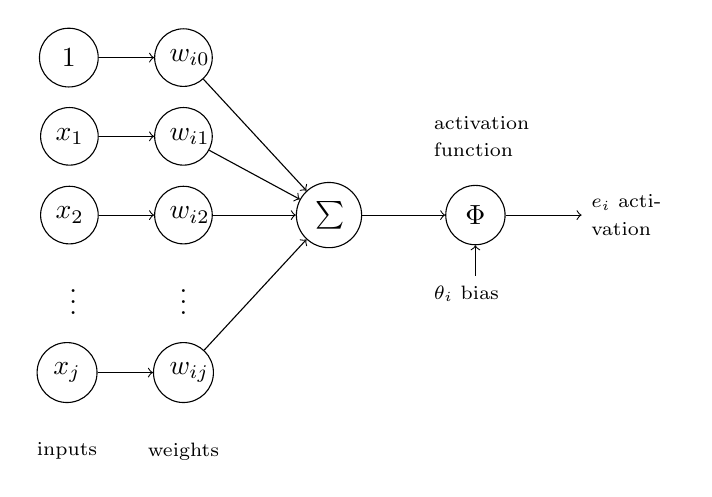
\begin{tikzpicture}
\tikzset{basic/.style={draw,fill=white!20,text width=1em,text badly centered}}
\tikzset{input/.style={basic,circle}}
\tikzset{weights/.style={basic,circle}}
\tikzset{functions/.style={basic,circle,fill=white!10}}
        \node[functions] (center) {};
        \node[above of=center,font=\scriptsize,text width=3em] {activation\\function};
        \node[functions](center){$\Phi$};
        \node[below of=center,font=\scriptsize,text width=3em](below) 
        {$\theta_i$~bias};
            \path[draw,->] (below) -- (center);
        \node[right of=center] (right) {};
        \node[right of=right,font=\scriptsize,text width=3em](output){$e_i$~activation};
            \path[draw,->] (center) -- (output);
        \node[functions,left=3em of center] (left) {$\sum$};
            \path[draw,->] (left) -- (center);
        \node[weights,left=3em of left] (2) {$w_{i2}$} -- (2) node[input,left=2em of 2] (l2) {$x_2$};
            \path[draw,->] (l2) -- (2);
            \path[draw,->] (2) -- (left);
        \node[below of=2] (dots) {$\vdots$} -- (dots) node[left=3em of dots] (ldots) {$\vdots$};
        \node[weights,below of=dots] (n) {$w_{ij}$} -- (n) node[input,left=2em of n] (ln) {$x_j$};
            \path[draw,->] (ln) -- (n);
            \path[draw,->] (n) -- (left);
        \node[weights,above of=2] (1) {$w_{i1}$} -- (1) node[input,left=2em of 1] (l1) {$x_1$};
            \path[draw,->] (l1) -- (1);
            \path[draw,->] (1) -- (left);
        \node[weights,above of=1] (0) {$w_{i0}$} -- (0) node[input,left=2em of 0] (l0) {$1$};
            \path[draw,->] (l0) -- (0);
            \path[draw,->] (0) -- (left);
        \node[below of=ln,font=\scriptsize] {inputs};
        \node[below of=n,font=\scriptsize] {weights};
    \end{tikzpicture}
    \caption[Modellneuron]{Simple model neuron with $x_j$ inputs and associated $w_{ij}$ weights. The activation function $\Phi$ determines the activation $e_i$ of the neuron from the total net input $\sum$ and, taking the bias $\theta_i$ into account.}
    \label{Modellneuron}
\end{figure}

\newpage

In \cref{Modellneuron} the structure of a single neuron is modelled. The \textit{activation $e_i$} results from the input signals $x_j$, with the respective \textit{weights} $w_{ij}$ and the additional \textit{non-linear characteristic} $\Phi$. The \textit{bias $\theta_i$} has a constant input $x_0 = 1$ with the weight $w_{0i}=-\theta_i$. The activation of a neuron thus can be formulated in the equation \cite{handbuch2013ki}:

%GLEICHUNG AKTIVIERUNG
\begin{equation}
e_i= \Phi \left(\sum_{j=0}^n w_{ij}*x_j + \theta_i\right)
\end{equation}

\section{Activation Functions}
The main functions used are the \textit{Logistic Sigmoid}, the \textit{Tangens Hyperbolicus (Tanh)} and the \textit{Rectified Linear Unit (ReLU)}. 

The sigmoid function has an s-shape as seen in \cref{Sigmoid}. It has its greatest gradient in the area around the threshold value and the interval [0,1] as the value range. This makes particularly large negative numbers 0 and large positive numbers 1. The sigmoid function is preferred as an activation function mainly because of its easy differentiability. With $z$ defined as the sum of all inputs $x_j$ with associated weights $w_{ij}$, the sigmoid function is given by the equation \cite{sigmoid}:


\begin{equation}
    \label{simple_equation}
    \phi(z)=\frac{1}{1+e^{-z}}
\end{equation}

The Tanh is visible in \cref{TanH}. Analogous to the sigmoid function, it is continuous, differentiable and bounded. The range is within the interval [-1,1]. Due to the negative interval the weight between two neurons is changed even if the preceding neuron is not activated, which makes the learning easier.

\begin{equation}
\phi(z)=tanh(z)=\frac{e^z-e^{-z}}{e^z+e^{-z}}
\end{equation}

\cref{ReLU} shows the ReLU function. All negative values become zero, which means that in this case the gradient is also zero and not all neurons are active simultaneously. However, it can also result in "dead" neurons that are never activated and therefore not playing any role in discriminating the input which makes them superfluous in the training process. The ReLU function is defined as the positive part of its argument:

\begin{equation}
\phi(z) = max(0,z)
        =\begin{cases} 
        0 & if~ z < 0 \\
        z & if~ z \geq\ 0
        \end{cases}
\end{equation}

To solve the problem of dead neurons there are modifications of the ReLU function like the \textit{Leaky ReLU}. Instead of setting all values at $z<0$ to zero, the slope for negative values is 0.1 \cite{activationfunction}.


%ABBILDUNG AKTIVIERUNGSFUNKTIONEN
\begin{figure}[h]
    \centering
	\subfigure[Logistic Sigmoid]{
    		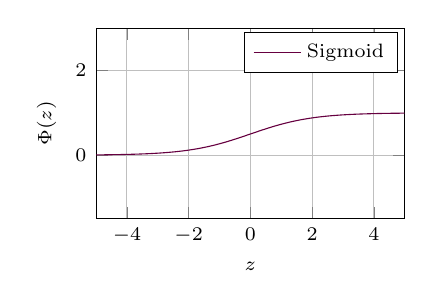
\begin{tikzpicture}
			\begin{axis}[width=5.5cm,height=4cm,ylabel=$\Phi(z)$,xlabel=$z$,ymin=-1.5,ymax=3,xmin=-5,xmax=5]
				\addplot[leuphy,smooth] {1/(1+exp(-x))};
				\addlegendentry{Sigmoid}
			\end{axis}
			\label{Sigmoid}
		\end{tikzpicture}
	}
	\subfigure[Hyperbolic Tangent]{
		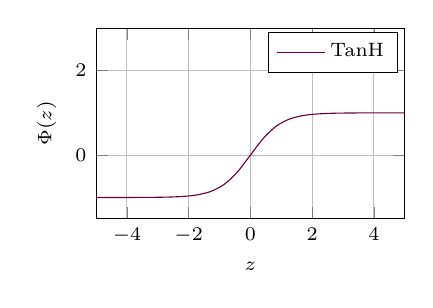
\begin{tikzpicture}
			\begin{axis}[width=5.5cm,height=4cm,ylabel=$\Phi(z)$,xlabel=$z$,ymin=-1.5,ymax=3,xmin=-5,xmax=5]
				\addplot[leuphy,smooth] {tanh(x)};
				\addlegendentry{TanH}
			\end{axis}
			\label{TanH}
		\end{tikzpicture}
	}
	\subfigure[Rectified Linear Unit]{
    		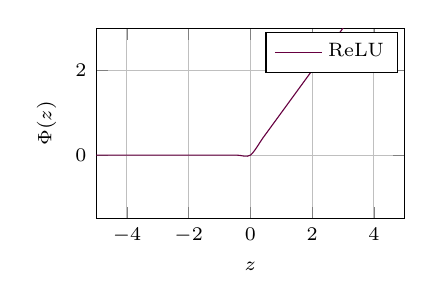
\begin{tikzpicture}
			\begin{axis}[width=5.5cm,height=4cm,ylabel=$\Phi(z)$,xlabel=$z$,ymin=-1.5,ymax=3,xmin=-5,xmax=5]
				\addplot[leuphy,smooth] {(x>=0)*x)};
				\addlegendentry{ReLU}
			\end{axis}
			\label{ReLU}
		\end{tikzpicture}
	}
\caption[Aktivierungsfunktionen]{The three most common activation functions in neural networks. The sigmoid function with an interval of [0,1], the TanH function [-1,1] and the ReLU function with a half-open interval [0,$\infty$[.}
\end{figure}


\section{Multilayer-Perceptron} \label{sec:training}

If several perceptrons are interconnected a so-called \textit{Multilayer-Perceptron (MLP)} is created. This always consists of one input-, one output-, and any number of hidden layers. There are two basic types of MLPs according to the network structure. The \textit{feed forward network (FFN)} and the \textit{recurrent network}. In FFNs the information is processed from front to back through the layers and the individual layers are connected with weights. In the case of the recurrent network, outputs are fed back to inputs through loops or directed circles \cite{computational2015intelligence}.


% %%NEURAL NETWORK
% \begin{figure}[h]
% 	\centering
% 	\begin{tikzpicture}[shorten >=1pt]
% 		\tikzstyle{unit}=[draw,shape=circle,minimum size=1.15cm]
% 		%\tikzstyle{hidden}=[draw,shape=circle,fill=black!25,minimum size=1.15cm]
% 		\tikzstyle{hidden}=[draw,shape=circle,minimum size=1.15cm]

% 		\node[unit](x0) at (0,3.5){$x_0$};
% 		\node[unit](x1) at (0,2){$x_1$};
% 		\node at (0,1){\vdots};
% 		\node[unit](xn) at (0,0){$x_N$};

% 		\node[hidden](h10) at (3,4){};
% 		\node[hidden](h11) at (3,2.5){};
% 		\node at (3,1.5){\vdots};
% 		\node[hidden](h1m) at (3,-0.5){};

% 		\node(h22) at (5,0){};
% 		\node(h21) at (5,2){};
% 		\node(h20) at (5,4){};
		
% 		\node(d3) at (6,0){$\ldots$};
% 		\node(d2) at (6,2){$\ldots$};
% 		\node(d1) at (6,4){$\ldots$};

% 		\node(hL12) at (7,0){};
% 		\node(hL11) at (7,2){};
% 		\node(hL10) at (7,4){};
		
% 		\node[hidden](hL0) at (9,4){};
% 		\node[hidden](hL1) at (9,2.5){};
% 		\node at (9,1.5){\vdots};
% 		\node[hidden](hLm) at (9,-0.5){};

% 		\node[unit](y1) at (12,3.8){$y_1$};
% 		\node[unit](y2) at (12,2){$y_2$};
% 		\node at (12,1){\vdots};	
% 		\node[unit](yc) at (12,0){$y_C$};

% 		\draw[->] (x0) -- (h11);
% 		\draw[->] (x0) -- (h1m);

% 		\draw[->] (x1) -- (h11);
% 		\draw[->] (x1) -- (h1m);

% 		\draw[->] (xn) -- (h11);
% 		\draw[->] (xn) -- (h1m);

% 		\draw[->] (hL0) -- (y1);
% 		\draw[->] (hL0) -- (yc);
% 		\draw[->] (hL0) -- (y2);

% 		\draw[->] (hL1) -- (y1);
% 		\draw[->] (hL1) -- (yc);
% 		\draw[->] (hL1) -- (y2);

% 		\draw[->] (hLm) -- (y1);
% 		\draw[->] (hLm) -- (y2);
% 		\draw[->] (hLm) -- (yc);

% 		\draw[->,path fading=east] (h10) -- (h21);
% 		\draw[->,path fading=east] (h10) -- (h22);
		
% 		\draw[->,path fading=east] (h11) -- (h21);
% 		\draw[->,path fading=east] (h11) -- (h22);
		
% 		\draw[->,path fading=east] (h1m) -- (h21);
% 		\draw[->,path fading=east] (h1m) -- (h22);
		
% 		\draw[->,path fading=west] (hL10) -- (hL1);
% 		\draw[->,path fading=west] (hL11) -- (hL1);
% 		\draw[->,path fading=west] (hL12) -- (hL1);
		
% 		\draw[->,path fading=west] (hL10) -- (hLm);
% 		\draw[->,path fading=west] (hL11) -- (hLm);
% 		\draw[->,path fading=west] (hL12) -- (hLm);
		
% 		\draw [decorate,decoration={brace,amplitude=10pt},xshift=-4pt,yshift=0pt] (-0.5,4) -- (0.75,4) node [black,midway,yshift=+0.6cm]{input layer};
% 		\draw [decorate,decoration={brace,amplitude=10pt},xshift=-4pt,yshift=0pt] (2.5,4.5) -- (3.75,4.5) node [black,midway,yshift=+0.6cm]{$1^{\text{st}}$ hidden layer};
% 		\draw [decorate,decoration={brace,amplitude=10pt},xshift=-4pt,yshift=0pt] (8.5,4.5) -- (9.75,4.5) node [black,midway,yshift=+0.6cm]{hidden layer};
% 		\draw [decorate,decoration={brace,amplitude=10pt},xshift=-4pt,yshift=0pt] (11.5,4.3) -- (12.75,4.3) node [black,midway,yshift=+0.6cm]{output layer};
% 	\end{tikzpicture}
% 	\caption[Feed Forward Network]{Simple feed forward network with $N$ input neurons, hidden neurons and $C$ output neurons}
% 	\label{Multilayer-Perzeptron}
% \end{figure}

For instance, when a network is used to solve a classification problem, typically one initial neuron per class is used, with additional layers allowing for more precise classification. However, the central step that gives a neural network its recognition capabilities is the training. During the training, the weights and biases of all neurons in the network are gradually adjusted so that it learns to map the inputs to the desired outputs. When training neural networks, a distinction is made between three basic learning methods: The \textit{supervised learning}, \textit{unsupervised learning} and \textit{reinforcement learning}. In supervised learning the results are known from a sample data set. These are repeatedly compared with the output of the untrained network and its adjusted accordingly so that after the training the network acts correctly in situations not present in the training data. Unsupervised learning is based solely on the input without the results to be achieved are known. Therefore, the aim of the network is to find the structure hidden in collections of usually a very large number of unlabeled data. The idea of reinforcement learning is learning by interacting with the environment, since in interactive problems it is often impractical to obtain examples of desired behaviour that are representative. Instead of trying to find hidden structure, reinforcement learning is about to identify which actions yield the most reward by trying them out. Through feedback in the form of rewards and punishments, the network looks for the actions that bring the most rewards over a longer period of time \cite{reinforce2018learning}. 



\section{Backpropagation} \label{sec:backpropagation}

One very common algorithm for supervised learning is the backpropagation. It is based on a gradient descent method and suitable for networks with several layers of trainable weights by finding the minimum of the error function. The gradient is a vector of the partial derivatives, which points in the direction of the steepest rise. This vector moves towards the minimum since it is multiplied by a negative step size (or learning factor).

By providing training data, a set of known pairs of input and output is given. At the beginning the parameters of the network are randomly selected and the output is generated by an initial forward propagation of an presented input. The output is then compared with the desired target from the training data and results in an error signal $\delta_{i}$. In a second phase of a backward pass through the network the model parameters (weights and biases) are adjusted. 

%Bei der Standard $\delta - Regel$ für einschichtige Netze ergibt sich der \textit{Einzelfehler} $E$ eines Trainingssamples nach einer Vorwärtspropagierung über $M$ Output-Neuronen aus

% \begin{equation}
%     E = 1/2 \sum_{m=1}^M (t_m - e_m)^2
% \end{equation}

% $t_m$ ist der gewünschte Output des Neurons $m$ und $e_m$ die Aktivität des Output-Neurons nach der Propagierung. Die Multiplikation mit $1/2$ dient der besseren Ableitung. Ziel des Verfahrens ist es, durch Anpassung der Gewichte den Gesamtfehler zu minimieren. Dazu werden die Einzelfehler jedes Trainingssamples partiell nach dem Gewicht abgeleitet. Der daraus resultierende Gradient ist ein Vektor, der in Richtung des stärksten Anstiegs zeigt und dessen Länge der Steigung entspricht. Zur Verringerung des Fehlers werden die Gewichte in die entgegengesetzte Richtung verändert, es gilt
% \begin{equation}
%     \Delta w_{ij} = \eta ~ \frac{\partial E_m}{\partial w_{ij}}
%     \label{eq:deltagewicht}
% \end{equation}
% Die Änderung des Gewichtes $\Delta w_{ij}$ ist immer proportional zur Steigung. Als $\eta$ wird die Änderungsgeschwindigkeit oder auch \textit{Lernrate} bezeichnet. Durch die zufällige Wahl der Initialgewichte ist die Lernrate zu Beginn relativ groß zu wählen, da zu erwarten ist, dass diese relativ weit entfernt von den Zielgewichten liegen. Später im Training sollte sie nicht zu groß gewählt werden, da sonst eventuell Minima übersprungen werden. Eine \textit{Epoch} bezeichnet den gesamten Durchlauf aller Trainingssamples. Nach jeder Epoche kann der \textit{Gesamtfehler F} angegeben werden. Er entspricht der Summe aller Einzelfehler.

% Wird die $\delta-Regel$ für Feed Forward Networks mit mehreren Hidden Layer und nicht-linearen Aktivierungsfunktionen angewendet, sind die Änderungen der Gewichte voneinander abhängig. Wie in \cref{Perzeptron} bereits vorgestellt, ist die Aktivierung eines Neurons definiert durch
% \begin{equation}
% e_i= \Phi \sum_{j=0}^n w_{ij}*x_j = \Phi(z)
% \end{equation}

% Aus \cref{eq:deltagewicht} und der Anwendung der Kettenregel, ergibt sich die Änderung des Gewichtes eines Neurons im mehrschichtigem Netz. Auf genauere Herleitungen wird an dieser Stelle verzichtet, da sie keine Relevanz für weitere Betrachtungen der vorliegenden Arbeit darstellt. Die Änderung $\Delta w_{ij}$ ergibt sich mit dem \textit{Fehlersignal} $\delta_i$ aus 
% \begin{equation}
%     \Delta w_{ij} = \eta ~ \delta_i ~ e_j
    
% \end{equation}

The two equations given below specify the error signal with the determination as a recursive process starting with the output units. If it is an output neuron, the error signal is not dependent on the previous neuron

\begin{equation}
     \delta_{pi} = \Phi_i^{\prime}(z)(t_{pi}- e_{pi})
 \end{equation}

where $t_{pi}$ is the target output for the $i$th component of the output of pair p and $e_{pi}$ is the $i$th element of the actual output produced. $\Phi_i^{\prime}(z)$ is the derivative of a semilinear activation function.

In case of a neuron in the hidden layer for which there is no specified target, the error signal is determined recursively in terms of the signals of the neuron to which it directly connects and the weights of those connections. With $k$ following neurons, the error signal is given by

\begin{equation}
    \delta_{pi} = \Phi_i^{\prime}(z)\sum_k \delta_{pk} w_{ik}
\end{equation}

%http://www.ra.cs.uni-tuebingen.de/lehre/ss06/pro_learning/MLPSchmiedl.pdf

It can be seen that derivation assumes differentiable non-linearity $\Phi$, which is why the backpropagation method can only be applied by using non-linear activation functions. When ReLU (\cref{ReLU}) is used as the activation function, the derivatiove $\Phi_i^{\prime}(z)$ is either 0 or 1, thus simplifying and accelerating the learning process \cite{back1986propagation}.

However, backpropagation is sometimes misunderstood as the full neural network learning algorithm, even though it is initially just a method for computing a gradient. Other algorithms, such as stochastic gradient descent or Adam, are used for the actual learning using the gradient provided with backpropagation \cite{Goodfellow-et-al-2016}.


% \section{Convolutional Neuronal Network} \label{sec:ConvNet}

% Convolutional Neural Networks ermöglichen es, einen Input in Form einer Matrix zu verarbeiten, mithilfe dessen das Erkennen von räumlichen Abhängigkeiten in einem Bild möglich ist. Ihr Ziel ist es, Bilder in eine leichter zu verarbeitende Form zu bringen, ohne dabei Features zu verlieren. Aus diesem Grund sind sie besonders gut geeignet für die Klassifizierung von Bildern. Verglichen dazu, benötigt ein normales MLP einen Vektor als Input, weshalb die Pixel eines Bildes in einer langen Kette hintereinander ausgerollt werden müssten (\textit{Flattening}). Gleiche Objekte in anderen Positionen hätten so unterschiedliche Input-Vektoren, weshalb Objekte nicht unabhängig von der Position im Bild erkannt werden können.

% Die wichtigsten Bestandteile eines CNNs sind die paarweise arbeitenden \textit{Convolutional} und \textit{Pooling Layer}. Sie sind für das Herausarbeiten von Features mit anschließender Komprimierung verantwortlich. Dieser Prozess wird fortlaufend durch die einzelnen Schichten weitergeführt. Üblicherweise sind die ersten Schichten für gröbere Informationen verantwortlich und mit zusätzlichen Schichten wird sich spezifischeren Features angenähert. Am Ende des Netzes wird mithilfe von Fully Connected und Softmax Layern die Klassifikation durchgeführt und die Wahrscheinlichkeiten ausgegeben.\cite{introduction2017dl} Der Aufbau des CNNs AlexNet ist in \cref{AlexNet} dargestellt.

% \begin{figure}[ht]
%   \centering
%   \includegraphics[width=\linewidth]{AlexNet.png}
%   \caption[AlexNet]{Visualisierung von AlexNet, mit fünf Convolution Layer und drei Fully Connected Layern. Max-Poolingschichten folgen jeweils nach dem ersten, zweiten und fünften Convolution Layer. (eigene Darstellung in Anlehnung an \cite{alex2017}}
%   \label{AlexNet}
% \end{figure}

% \textbf{Convolutional Layer.}
% Convolution Layer sind der Kern eines CNN. Jedes Neuron des Convolutional Layer hat eine feste Verbindung zu Neuronen eines Bereichs des vorherigen Layers (bzw. des Input-Bildes) der als \textit{Receptive Field} bezeichnet wird. Dadurch werden die Merkmale mit ihrer räumlichen Position im Bild verbunden. Die Input-Matrix wird mit einer vorher festgelegten Anzahl \textit{Filtern} analysiert. Das Ergebnis nach Anwendung des Filters ist der gewichtete Input. Dieser wird anschließend im Convolution Layer gespeichert. Durch die Anpassung seiner Gewichte wird der Layer darauf trainiert, das Bild auf bestimmte Features zu untersuchen. Die Filter haben eine feste Pixelgröße, die auch als \textit{Kernel-Size} bezeichnet wird. Für die Filterung des kompletten Bildes wird eine konstante Schrittweite des Filters definiert, die auch \textit{Stride} genannt wird. Die Methode, die vorgibt, wie sich der Filter am Rand der Matrix verhalten soll heißt \textit{Padding}. Für jedes Feature entsteht eine Ergebnismatrix, die \textit{Feature- oder Kernel-Map}. Die Tiefe des Convolutional Layer entspricht der Anzahl Feature-Maps. Die Dimensionen der Feature-Map sind abhängig von den Hyperparametern Padding, Stride und dem Receptive Field. In \cref{Convolution} ist eine Convolution Operation gezeigt. Eine $7~x~7$ - Matrix wird mit einem Filter der Kernel-Size $3~x~3$, Stride 1, ohne Padding gefaltet. \cite{convolutional} Die 4 aus der Ergebnismatrix ergibt sich beispielsweise durch: $4 = 1*1+0*0+0*1+1*0+1*1+0*0+1*1+1*0+1*1 = 1+1+1+1$ 
% \\

% % CONVOLUTIONAL LAYER 
% \begin{figure}[ht]
%     \centering
% \newcommand\numRowsK{3}
% \newcommand\numColsK{3}
% \newcommand{\K}[2]{% #1: row, #2: col
%     \edef\Kcol##1##2##3{###2}%
%     \edef\Krow##1##2##3{\noexpand\Kcol###1}%
%     \Krow
%         {1 0 1}
%         {0 1 0}
%         {1 0 1}%
% }

% \begin{tikzpicture}
%     % ------- style -------
%     \tikzset{%
%         parenthesized/.style={%
%             left delimiter  = (,
%             right delimiter = ),
%         },
%         node distance = 10mu,
%     }

%     % ------- equation -------
%     \matrix[matrix of math nodes, parenthesized] (I) {
%         0 & 1 & 1 & 1 & 0 & 0 & 0 \\
%         0 & 0 & 1 & 1 & 1 & 0 & 0 \\
%         0 & 0 & 0 & 1 & 1 & 1 & 0 \\
%         0 & 0 & 0 & 1 & 1 & 0 & 0 \\
%         0 & 0 & 1 & 1 & 0 & 0 & 0 \\
%         0 & 1 & 1 & 0 & 0 & 0 & 0 \\
%         1 & 1 & 0 & 0 & 0 & 0 & 0 \\
%     };

%     \node (*) [right = of I] {${}*{}$};

%     \newcommand\Kmatrix{}
%     \foreach \row in {1, ..., 3} {
%         \gdef \sep {}
%         \foreach \col in {1, ..., 3} {%
%             \xdef \Kmatrix {\unexpanded\expandafter{\Kmatrix}\unexpanded\expandafter{\sep}\noexpand \K{\row}{\col}}
%             \gdef \sep { \& }
%         }
%         \xdef \Kmatrix {\unexpanded\expandafter{\Kmatrix}\noexpand\\}
%     }
%     \matrix[matrix of math nodes, parenthesized, ampersand replacement=\&] (K) [right = of *] {
%         \Kmatrix
%     };

%     \node (=) [right = of K] {${}={}$};

%     \matrix[matrix of math nodes, parenthesized] (I*K) [right = of {=}] {
%         1 & 4 & 3 & 4 & 1 \\
%         1 & 2 & 4 & 3 & 3 \\
%         1 & 2 & 3 & 4 & 1 \\
%         1 & 3 & 3 & 1 & 1 \\
%         3 & 3 & 1 & 1 & 0 \\
%     };

%     % ------- highlighting -------
%     \newcommand\rowResult{1}
%     \newcommand\colResult{4}

%     \begin{scope}[on background layer]
%         \newcommand{\padding}{2pt}
%         \coordinate (Is-nw) at ([xshift=-\padding, yshift=+\padding] I-\rowResult-\colResult.north west);
%         \coordinate (Is-se) at ([xshift=+\padding, yshift=-\padding] I-\the\numexpr\rowResult+\numRowsK-1\relax-\the\numexpr\colResult+\numColsK-1\relax.south east);
%         \coordinate (Is-sw) at (Is-nw |- Is-se);
%         \coordinate (Is-ne) at (Is-se |- Is-nw);

%         \filldraw[leuphy,  fill=leuphy!10!white] (Is-nw) rectangle (Is-se);
%         \filldraw[leuphy,  fill=leuphy!10!white] (I*K-\rowResult-\colResult.north west) rectangle (I*K-\rowResult-\colResult.south east);

%         \draw[thick,leuphy, dotted] 
%             (Is-nw) -- (K.north west)
%             (Is-se) -- (K.south east)
%             (Is-sw) -- (K.south west)
%             (Is-ne) -- (K.north east)
%         ;
%         \draw[thick,leuphy, dotted] 
%             (I*K-\rowResult-\colResult.north west) -- (K.north west)
%             (I*K-\rowResult-\colResult.south east) -- (K.south east)
%             (I*K-\rowResult-\colResult.south west) -- (K.south west)
%             (I*K-\rowResult-\colResult.north east) -- (K.north east)
%         ;

%         \draw[leuphy,  fill=leuphy!10!white] (K.north west) rectangle (K.south east);
                
%     \end{scope}

%     % ------- labels -------
%     \tikzset{node distance=0em}
%     \node[below=of I] (I-label) {$I$};
%     \node at (K |- I-label)     {$K$};
%     \node at (I*K |- I-label)   {$I*K$};
% \end{tikzpicture}%
%     \caption[Convolutional Layer]{Die Faltung der $7~x~7$ Matrix $I$ mit einem $3~x~3$ Filter $K$, ohne Padding und Stride 1 ergibt die Ergebnismatrix $I * K$}
% 	\label{Convolution}
% \end{figure}

% \textbf{Pooling Layer.}
% Die Aufgabe der Pooling Schicht ist es, die räumliche Auflösung der Feature Maps zu minimieren, sodass die Anzahl der Gewichte und damit der Rechenaufwand reduziert wird. Zusätzlich beugt sie der Überanpassung \textit{Overfitting} vor. Overfitting beschreibt eine zu hohe Anpassen des Netzes an die Trainingsdaten, weches das Erkennen eines allgemeingültigen Musters wiederum verhindert. Um die Features in einer kleineren Darstellung zu erhalten, werden weniger signifikante Daten auf Kosten der räumlichen Auflösung verworfen. Die gängigsten Arten sind das Max-Pooling und das Average-Pooling Verfahren. Bei beiden Verfahren läuft ein Fenster fester Größe mit einer bestimmten Schrittgröße jede, nach dem Convolutional Layer entstandene, Feature Map ab und verkleinern diese. Beim Max-Pooling wird der höchste Wert verwendet, beim Average-Pooling wird der Mittelwert aller Werte genutzt. In \cref{Pooling} ist die Arbeitsweise des Max-Pooling Verfahrens dargestellt. \cite{convolutional}\\

% \begin{figure}[htbp]
%   \centering
%     \includegraphics[width=.7\linewidth,trim={0 0.2 0 1.4cm},clip]{maxpool.jpeg}
%     \caption[Pooling Layer]{Jede 2x2 Teilmatrix wird durch ihren maximalen Eintrag ersetzt. Die Schrittgröße ist 2, weshalb es sich um non-overlapping Pooling handelt.}
%   \label{Pooling}
% \end{figure}

% \textbf{Fully Connected Layer.}
% Auf die Convolutional und Pooling Layer folgen Fully Connected Layer (FC). Neuronen des FC sind mit allen Neuronen der vorherigen Schicht verbunden und ähneln der Architektur eines einfachen mehrschichtiges Perzeptrons. Der Flattening Prozess transformiert den mehrdimensionale Output des vorherigen Layers in einen eindimensionalen Merkmalsvektor. Der Fully Connected Layer ist wie der Convolutional Layer trainierbar, er multipliziert den Input mit einer Gewichts-Matrix und addiert einen Bias-Vektor. Diese Parameter sind trainierbar. Bei der Klassifikation muss die Outputsize des letzten FC der Anzahl Klassen des Datensatzes entsprechen.\cite{FullyConnected} 

% \textbf{Softmax Layer.}
% Der Softmax Layer befindet sich am Ende eines CNN und wendet eine Softmax Funktion an. Die Dimensionalität entspricht bereits der Anzahl an Objektklassen, die Werte können jedoch beliebig sein. Er transformiert die Werte des Vektors aus dem letzten FC, korrespondierend zu der Höhe ihrer vorherigen Werte, in den Wertebereich [0, 1]. Aufaddiert ergeben die neuen Werte 1, sodass Werte einer Wahrscheinlichkeitsverteilung entstehen. Wenn $z_j$ ein Wert aus dem Vektor $z$ mit $1~x~K~Werten$, dann ergibt sich der transformierte Wert $\sigma(z)_j$ aus \cite{introduction2017dl}:
% \begin{align}
% \begin{split}
% \sigma(z)_j = \frac{e^{z_j}}{\sum_{k=1}^K e^{z_k}} ~~~~~~~
% j = 1,...K \quad \\
% mit ~~ 0 \leq \sigma(z)_j \leq 1 ~~~~~~~ und ~~ \sum_{k=1}^K \sigma_k = 1 
% \end{split}
% \end{align}

\addcontentsline{toc}{chapter}{Bibliography}
\printbibliography %[title=References] %To change title of the bibliography

\end{document}